\documentclass[11pt,a4paper,twocolumn]{IEEEtran}
\usepackage[utf8]{inputenc}
\usepackage{lipsum}
\usepackage{tabularx, booktabs}
\usepackage{amsmath}
\usepackage{amsfonts}
\usepackage{caption}
\usepackage{pdfpages}
\usepackage[margin=2.5cm]{geometry}
\usepackage{listings,lstautogobble}
\usepackage{amssymb}
\usepackage{hyperref}
\usepackage{graphicx}
\usepackage{svg}
\usepackage{pgf}
\usepackage{array}
\usepackage{cancel}
\usepackage{lipsum}
\usepackage{tikz}

\newcommand*\circled[2][1.6]{\tikz[baseline=(char.base)]{
		\node[shape=circle, draw, inner sep=1pt, 
		minimum height={\f@size*#1},] (char) {\vphantom{WAH1g}#2};}}
\newcommand{\sepline}{\noindent\makebox[\linewidth]{\rule{\textwidth}{1.2pt}}}
\newcommand{\bsepline}{\noindent\makebox[\linewidth]{\rule{7.5cm}{1.2pt}}}
\newcommand{\esepline}{\noindent\makebox[\linewidth]{\rule{7.5cm}{0.5pt}}}

\newcommand{\mysvg}[2]{\includesvg[width=0.#2\linewidth]{../svgs/#1}}
\newcommand*{\Scale}[2][4]{\scalebox{#1}{$#2$}}
\definecolor{RoyalBlue}{cmyk}{1, 0.50, 0, 0}
\lstset{language=Python,
	keywordstyle=\color{RoyalBlue},
	basicstyle=\fontsize{10}{10}\ttfamily,
	commentstyle=\ttfamily\itshape\color{gray},
	stringstyle=\ttfamily,
	showstringspaces=false,
	breaklines=true,
	frameround=ffff,
	rulecolor=\color{black},
	autogobble=true
}

\author{Saverio Monaco\\ \sepline}
\title{\textbf{Low Pass FIR Filter in FPGA}}

\begin{document}
	\maketitle
	\begin{abstract}
		FIR Filters are a class of filters that are relatively easy to implement in a FPGA. They can be pretty versatile since they can comprehend Low Pass, High Pass, Band Stop and Band Pass filters. In this project we present an example of a Low Pass filter.
	\end{abstract}
	\section{FIR Filter}
		A Filter takes as an input a signal $X[n]$ and outputs a refined one $Y[n]$, for the case of a FIR Filter, the law $X[n]\to Y[n]$ is described as follows: 
		$$ Y[n] = \sum_{i=0}^N C_i x[n-i] $$
		where $N$ is the filter order. This order is totally arbitrary, the higher the order is, the better the filter performs. In this project, we choosed to implement a 3 order filter.\\ Then our transformation law is
		$$\begin{aligned} Y[n]&=\sum_{i=0}^3 C_ix[n-i]=\\ & \Scale[0.8]{\hspace*{.2cm}=C_0x[n]+C_1x[n-1]+C_2x[n-2]+C_3x[n-3]}\end{aligned}$$
		The circuit able to implement this is the following:
		\begin{figure}[h]
			\centering
			\includegraphics[width=1\linewidth]{img/FIR_direct}
		\end{figure}\\
		The component represented by a square is a \textbf{Flip-flop}, while \includegraphics[width=0.05\linewidth]{img/x} and \includegraphics[width=0.05\linewidth]{img/+} represent respectively the operations of multiplication and addition.
		\subsection*{Flip-flop}
		A Flip-flop is one of the most common component found in a FPGA, by itself it can be seen as a simple component for memory storage, although it can be implemented in more complex architectures like a FIR Filter as we will see.\newpage
		\begin{figure}[h]
			\centering
			\includegraphics[width=0.6\linewidth]{img/ff}
		\end{figure}
		In a flipflop we have two input signals and one output signal. The inputs are the data and the clock (represented by a periodic square wave function), what the flipflop basically does is checking at \emph{every rising edge of the clock} the value of D (data-in) and it mirrors it to Q (data-out). Here is an example:\\
	\begin{figure}[h]
		\centering
		\includegraphics[width=1\linewidth]{img/ffsignals}
	\end{figure}
		\subsection*{Operations in the circuit} Through the line of code
		\texttt{use ieee.numeric\_std.all;} we can implement additions and multiplications in our code. The main problem is handling multiplications with number less than 1, since we can only do moltiplications only with integers, for example: $$20\times 0.75 = 15$$ In binary terms it means
		$$ 10100_2 \times 0.11_2 = 1111_2$$
		To realize this, we must scale the quantity $0.11_2$ by multiplying it by $2^Q$ (resulting in a shift of bits) until we obtain an integer, then after the multiplication we can rescale back (shifting to the other direction).
		$$0.11_2 *\times 2^3 = 0.11_2 <<3 = 110$$
		Now we can do the multiplication
		$$10100_2\times 110_2 = 1111000_2$$
		Then we rescale back
		$$1111000_2 >> 3 = 1111_2 = 15$$
		\subsection*{The Coefficients $C_i$}
		The value of the coefficients depends on what type of filter do we want to implement and which value of frequencies do we want to filter out.\\
		The values of the coefficients can be computed with \emph{Python} using the function \texttt{firwin} in Scipy:\\
		\begin{lstlisting}
		from scipy import signal
		
		numtaps = 4
		f = 0.1
		
		signal.firwin(numtaps, f)
		
		array([0.04566357, 0.45433643, 0.45433643, 0.04566357])
		\end{lstlisting}
		The coefficients in output will make us build a low pass filter with a cut-off frequency of 0.1.
		\begin{figure}[h]
			\centering
			\includegraphics[width=0.7\linewidth]{img/lowpass}
		\end{figure}
	\section{Implementation of a FIR Filter in VHDL}
		To build a FIR Filter, we need first to build a flipflop. The total of \emph{entities} we need are then 4:
		\begin{itemize}
			\item flipflop
			\item flipflop\_sum (the final flipflop requires a bigger \texttt{std\_logic\_vector} as an output)
			\item fir\_filter\_4
			\item fir\_filter\_4\_tb (the testbench able to read from a .txt file and write in another .txt file the output signal, already provided)
		\end{itemize}
		In particular, the entity fir\_filter\_4 is defined as follows:\medskip\\
		\begin{tabular}{ll}
	clk	&	 : in std\_logic; \\
	rst	&	 : in std\_logic; \\
	c\_0	&	 : in std\_logic\_vector(7 downto 0); \\
	c\_1	&	 : in std\_logic\_vector(7 downto 0); \\
	c\_2	&	 : in std\_logic\_vector(7 downto 0);\\
	c\_3	&	 : in std\_logic\_vector(7 downto 0); \\
	data\_in	&	 : in std\_logic\_vector(7 downto 0); \\
	data\_out	&	 : out std\_logic\_vector(9 downto 0); \\
		\end{tabular}
	\section{The UART}
	A UART is one of the simplest hardware devices capable of transfer data from and to the FPGA:
	\begin{figure}[h]
		\centering
		\includegraphics[width=0.8\linewidth]{img/simpleuart.png}
	\end{figure}
	To set up a UART correctly, the device and the FPGA must agree on how quickly the data is transfered, this speed is called \emph{Baud rate}.\\
	The data stream is the following:
	\begin{figure}[h]
		\centering
		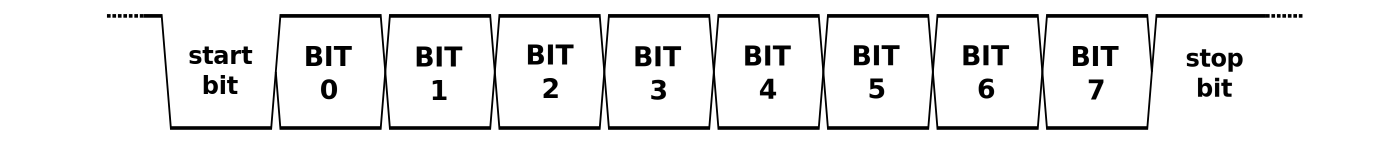
\includegraphics[width=1\linewidth]{img/UART_timing_diagram.pdf}
	\end{figure}\\
	By default the \emph{Idle state} (the state where the transmitter is waiting for data to send) is \texttt{HIGH}, the \emph{start bit} is \texttt{LOW}, no information is transfered with the start bit, it just tells that some data will be transfered after. Then the bits will be transfered, obviously they can be either 0 or 1, then the end of the stream is announced by the \emph{stop bit} that is \texttt{HIGH}\medskip\\
	The complete project can be schematized as it follows:
	\begin{figure}[h]
		\centering
		\includegraphics[width=1\linewidth]{img/projectcomplete}
	\end{figure}\\
	Inside the FPGA we will have a \emph{receiver} that will receive data from Python through a USB, the data will be sent to the FIR Filter, it will be filtered and then sent to the transmitter, from there Python can read the output.\\
	For this project we need then 3 main entities: the Fir Filter (already explained), the Receiver and the Transmitter (already provdided). These 3 entities are managed by another entity \emph{top}:
	\begin{figure}[h]
		\centering
		\hspace*{-.8cm}\includegraphics[width=1.1\linewidth]{img/code1.png.pdf}
	\end{figure}
	
	\section{Results}
	Using the Python library scipy.signal, it was possible to simulate the behaviour of a FIR Filter and compare the result with the one implemented in the FPGA:\\
	First we get the coefficients with the function \texttt{firwin} already explained:
	\begin{lstlisting}
		coefficients = signal.firwin(3, 0.1)
	\end{lstlisting}
	Where 3 is the number of taps, and 0.1 is the cutoff frequency.\\
	We load the signal from a .txt file
	\begin{lstlisting}
		signal = np.loadtxt("input.txt", dtype=np.int)
	\end{lstlisting}
	And then we filter this signal using the following code:
	\begin{lstlisting}
	filtered_signal = lfilter(coefficients, 1.0, signal)
	\end{lstlisting}
	The output is an array of \emph{floats} (and not integers like the output of the FPGA program) of the same lenght of the array \texttt{signal}. Those represents the points that are filtered.\\
	The difference between the performances of the two filters can be explained by some approximation error due to truncation, in fact the FPGA can only output integers and the approximation during the multiplications in the FPGA.\\
	The following scatter plot represent the filtered points using both filters: blue points are the ones filtered using Python, the red ones using the VHD code:
	\begin{figure}[h]
		\centering
		\includegraphics[width=1\linewidth,height=3.5cm]{img/index}
	\end{figure}
	
\end{document}